%==============================================================================
%  MATH 231 -- Linear Algebra I (Queens College, Fall 2026)
%  COMPUTATIONAL UNIT, PART 3 -- k-Means Clustering
%
%  Section numbering runs CONTINUOUSLY across the parts of the computational
%  unit:
%
%      Part 1  MATH231_computational_1_operation_counting        Sections 1-4
%      Part 2  MATH231_computational_2_k_nearest_neighbours      Sections 5-10
%      Part 3  MATH231_computational_3_k_means_clustering        Sections 11-15
%
%  Hence \setcounter{section}{10}: this part opens at Section 11.  References to
%  Sections 1-10 point into Parts 1-2.  Cross-references OUT of the unit still
%  name the unit ("the vector unit, Sec. 24.3").
%
%  STATUS: complete.  Sections 11-15.
%
%  AUDIENCE: distributed to students.  Keep it free of instructor-facing
%  apparatus -- time budgets, pacing notes, teaching cues.
%
%  SEC. 11.5 IS THE LOAD-BEARING RESULT and the reason the definitions in 11.2-
%  11.4 come before the algorithm rather than inside it.  The identity
%
%      sum_i ||x_i - c||^2  =  sum_i ||x_i - mu||^2 + m ||mu - c||^2
%
%  is what makes Lloyd's update step correct: it says the mean is the UNIQUE
%  minimiser of the within-cluster sum of squares, so line 8 of the pseudocode
%  is not a plausible heuristic but the exact solution of a subproblem.  The
%  proof is three lines and uses only the vector unit's expansion of
%  ||u+v||^2 (Sec. 24.3) plus the fact that sum_i (x_i - mu) = 0.  Sec. 12.4
%  then reuses it to prove termination.  If this theorem goes, the whole
%  document loses its spine.
%
%  MEAN vs CENTROID vs MEDOID.  These are separated deliberately in 11.2-11.4
%  and tabulated in 11.6, because students routinely use them interchangeably.
%  mu is the arithmetic object, the centroid is that object read as a point of
%  the space, and the medoid is a genuinely different thing -- it must BE a
%  member of the set, and it minimises total distance rather than total SQUARED
%  distance.  The geometric median is named in 11.6 only to complete the
%  three-way contrast; it is not used anywhere.
%
%  THE WORKED EXAMPLE in Sec. 12.5 is initialised DELIBERATELY BADLY -- both
%  starting centroids sit inside the left-hand cluster -- so that the run takes
%  two real iterations and visibly recovers.  A good initialisation converges in
%  one step and demonstrates nothing.  J drops 72.25 -> 2.67 across the run,
%  which is the number Sec. 12.4's monotonicity claim is checked against.
%
%  ELKAN'S LEMMA in Sec. 15.2 is stated with its one-line proof on purpose: it
%  is the metric axiom M4 of the vector unit doing measurable computational
%  work, and it is the same trick flagged in Part 2, Sec. 10.2.
%
%  Compile with pdflatex (standard TeX Live packages only; uses tikz).
%==============================================================================
\documentclass[11pt]{article}

\usepackage[margin=1in]{geometry}
\usepackage{amsmath,amssymb,amsthm}
\usepackage[dvipsnames]{xcolor}
\usepackage{enumitem}
\usepackage{booktabs}
\usepackage{array}
\usepackage[hidelinks]{hyperref}
\usepackage{titlesec}
\usepackage{needspace}
\usepackage{tikz}
\usetikzlibrary{arrows.meta,shapes.geometric}

%------------------------------------------------------------------ style ----
\titleformat{\section}{\large\bfseries\sffamily}{\thesection.}{0.6em}{}
\titleformat{\subsection}{\normalsize\bfseries\sffamily}{\thesubsection.}{0.5em}{}
\titlespacing*{\section}{0pt}{14pt}{6pt}

\theoremstyle{plain}
\newtheorem{thm}{Theorem}[section]
\newtheorem{lem}[thm]{Lemma}

\theoremstyle{definition}
\newtheorem{defn}{Definition}[section]
\newtheorem{ex}{Example}[section]
\theoremstyle{remark}
\newtheorem*{rmk}{Remark}
\newtheorem*{warn}{A common confusion}

\newcommand{\lookahead}{\par\smallskip\noindent
  \textbf{\sffamily\textcolor{RoyalBlue}{Looking ahead.}}\ \ignorespaces}
\newcommand{\lookback}{\par\smallskip\noindent
  \textbf{\sffamily\textcolor{ForestGreen}{From the vector unit.}}\ \ignorespaces}

%--------------------------------------------------------------- notation ----
\newcommand{\R}{\mathbb{R}}
\newcommand{\vc}[1]{\mathbf{#1}}
\newcommand{\norm}[1]{\lVert #1\rVert}
\newcommand{\X}{\mathcal{X}}
\newcommand{\Cl}{\mathcal{C}}
\newcommand{\bmu}{\boldsymbol{\mu}}
\DeclareMathOperator*{\argmin}{arg\,min}
\DeclareMathOperator*{\argmax}{arg\,max}

%--------------------------------------------------------------- pseudocode --
\newcommand{\kw}[1]{\textsf{\bfseries #1}}
\newcommand{\ind}{\hspace*{1.3em}}
\newcommand{\indd}{\hspace*{2.6em}}
\newcounter{algoline}
\newenvironment{algo}[2]{%
  \par\medskip\needspace{8\baselineskip}%
  \begin{center}\begin{minipage}{0.94\textwidth}%
  \hrule height 0.9pt \vspace{3pt}%
  \noindent{\sffamily\bfseries #1}\par\vspace{2pt}%
  \noindent{\small #2}\par\vspace{3pt}%
  \hrule height 0.4pt \vspace{5pt}%
  \begin{list}{\textbf{\arabic{algoline}:}}%
    {\usecounter{algoline}\setlength{\leftmargin}{2.3em}%
     \setlength{\labelwidth}{1.8em}\setlength{\labelsep}{0.5em}%
     \setlength{\itemsep}{2pt}\setlength{\topsep}{0pt}%
     \setlength{\parsep}{0pt}}%
}{%
  \end{list}\vspace{5pt}\hrule height 0.9pt%
  \end{minipage}\end{center}\medskip%
}

%------------------------------------------------------------- tikz helpers --
\tikzset{
  axisline/.style = {->, gray!75, thin},
  opbox/.style    = {draw=gray!65, rounded corners=2pt, fill=gray!8,
                     inner sep=5pt, font=\small, minimum height=8mm},
  opar/.style     = {-{Stealth[length=2.4mm,width=1.8mm]}, gray!80, thick},
  dpt/.style      = {circle, draw=gray!70, fill=gray!25, inner sep=0pt,
                     minimum size=5.4pt},
  c1pt/.style     = {circle, draw=RoyalBlue, fill=RoyalBlue!70, inner sep=0pt,
                     minimum size=5.4pt},
  c2pt/.style     = {circle, draw=BrickRed, fill=BrickRed!70, inner sep=0pt,
                     minimum size=5.4pt},
  cen1/.style     = {star, star points=5, draw=RoyalBlue, fill=RoyalBlue!85,
                     inner sep=0pt, minimum size=9pt},
  cen2/.style     = {star, star points=5, draw=BrickRed, fill=BrickRed!85,
                     inner sep=0pt, minimum size=9pt}
}

\title{\vspace{-1.2cm}\textbf{\sffamily MATH 231 -- Linear Algebra I}\\[4pt]
       {\large\sffamily The Computational Unit, Part 3 \textbullet\
        $k$-Means Clustering}\\[2pt]
       {\normalsize\sffamily Kiely Hall 326 \textbullet\
        Instructor: Kevin Bedoya}}
\author{}
\date{}

\begin{document}
\setcounter{section}{10}  % this part opens at Section 11; see the header note
\maketitle
\vspace{-1.6cm}

\noindent\textbf{About this document.} Part 2 placed a new point into groups
that were already known. This part has no groups and no labels: the data arrives
as a bare set of vectors, and the task is to find the structure in it. One new
object is needed --- the mean of a set of vectors --- and \S11 builds it before
the algorithm that uses it.

\begin{center}
\renewcommand{\arraystretch}{1.2}
\begin{tabular}{@{}l l l@{}}
\toprule
\textbf{Part} & \textbf{Sections} & \textbf{Subject} \\
\midrule
1 & \S1--\S4    & operation counting, Big-O, floating point, error \\
2 & \S5--\S10   & $k$-nearest neighbours \\
3 & \S11--\S15  & $k$-means clustering \\
\bottomrule
\end{tabular}
\end{center}

\begin{warn}[Whose \S11 is this?]
Section numbering runs continuously through the computational unit, so a bare
``\S7.4'' below means \S7.4 \emph{of this unit} --- Part 2. References into the
vector unit or the matrix unit always name them.
\end{warn}

\medskip
\noindent\textbf{Assumed.} From the vector unit: $\R^{n}$, addition and scalar
multiplication (\S24.2); the Euclidean norm and distance (\S2, \S14.2); the
metric axioms, in particular the triangle inequality \textbf{M4} (\S14.1);
$\langle\vc{u},\vc{u}\rangle=\norm{\vc{u}}^{2}$ and the expansion
$\norm{\vc{u}+\vc{v}}^{2}=\norm{\vc{u}}^{2}+2\langle\vc{u},\vc{v}\rangle
+\norm{\vc{v}}^{2}$ (\S24.3). From this unit: Big-O (\S2.7), FLOPs (\S4.6),
feature vectors and datasets (\S5.1), the squared-distance shortcut (\S7.5),
and the distinction between classification and clustering (\S9.1).

\medskip
\noindent\textbf{What you should be able to do afterwards.} State the clustering
problem; define the mean $\bmu$ of a set of vectors, the centroid and the
medoid, and say how they differ; prove that the mean minimises the sum of
squared distances; write down the $k$-means objective; run Lloyd's algorithm by
hand and write its pseudocode; explain why it terminates and why it may still
give a poor answer; count its operations and give its complexity; and name the
standard initialisation and speed-ups used in practice.

%==============================================================================
\section{Clustering, and the mean of a set of vectors}
%==============================================================================
%------------------------------------------------------------------------------
\subsection{The problem}
%------------------------------------------------------------------------------
\begin{quote}
Given a set of vectors $\X=\{\vc{x}_1,\dots,\vc{x}_N\}\subseteq\R^{n}$ and an
integer $k$, partition $\X$ into $k$ groups so that points in the same group are
close to one another and points in different groups are far apart.
\end{quote}

\noindent Compare that with \S5.2. There is no $\vc{q}$, because we are not
asking about a new point; there are no labels $y_i$, because nobody has told us
what the groups are. The output is not a prediction but a \textbf{partition} of
the data itself.

\begin{defn}[Clustering]
A \textbf{clustering} of $\X$ into $k$ parts is a partition
$\Cl_1,\dots,\Cl_k$ of $\X$: every $\vc{x}_i$ belongs to exactly one $\Cl_j$,
and no $\Cl_j$ is empty. Each $\Cl_j$ is a \textbf{cluster}. Equivalently it is
an \textbf{assignment} function $a:\{1,\dots,N\}\to\{1,\dots,k\}$, with
$\Cl_j = \{\,\vc{x}_i : a(i)=j\,\}$.
\end{defn}

\noindent Two things must be made precise before there is an algorithm: what
``close to one another'' means numerically --- \S12.1 --- and what a cluster's
\emph{centre} is, which is the rest of this section.

%------------------------------------------------------------------------------
\subsection{The mean of a set of vectors}
%------------------------------------------------------------------------------
The average of a list of numbers is familiar. The same definition works one slot
at a time on vectors, and it is nothing more than the arithmetic of the vector
unit applied to $m$ vectors at once.

\begin{defn}[Mean of a set of vectors]
Let $S=\{\vc{x}_1,\dots,\vc{x}_m\}\subseteq\R^{n}$ be non-empty. Its
\textbf{mean} is the vector
\[
  \bmu(S)
  \;=\; \frac{1}{m}\sum_{i=1}^{m}\vc{x}_i
  \;\in\; \R^{n} .
\]
When $S$ is understood we write simply $\bmu$.
\end{defn}

\noindent Unpacking that: the sum is $m-1$ vector additions, and dividing by $m$
is scalar multiplication by $1/m$, so $\bmu$ is a linear combination of the
$\vc{x}_i$ with every weight equal to $1/m$. Slot by slot,
\[
  \bmu
  = \Bigl[\ \frac{1}{m}\sum_{i=1}^{m}x_{i1},
    \ \ \frac{1}{m}\sum_{i=1}^{m}x_{i2},
    \ \ \dots,
    \ \ \frac{1}{m}\sum_{i=1}^{m}x_{in}\ \Bigr],
\]
which says the mean vector is the vector of the componentwise means: average the
first coordinate of everything, average the second, and so on. Nothing new is
happening in each slot; what is new is doing all $n$ of them at once and
regarding the result as a single point.

\begin{ex}
For $S=\{[\,1,1\,],\ [\,2,1\,],\ [\,1,2\,]\}$ in $\R^{2}$,
\[
  \bmu
  = \tfrac13\bigl([\,1,1\,]+[\,2,1\,]+[\,1,2\,]\bigr)
  = \tfrac13[\,4,\,4\,]
  = \bigl[\,\tfrac43,\ \tfrac43\,\bigr] .
\]
Note that $\bmu\notin S$: the mean of three points of the set is not one of
them. \hfill$\blacksquare$
\end{ex}

\noindent One identity is used twice below and is worth recording now. Summing
the deviations from the mean gives zero:
\[
  \sum_{i=1}^{m}(\vc{x}_i - \bmu)
  \;=\; \sum_{i=1}^{m}\vc{x}_i \;-\; m\bmu
  \;=\; m\bmu - m\bmu
  \;=\; \vc{0} ,
\]
which is just the definition of $\bmu$ rearranged. It says the mean sits at
the balance point of the set: the displacements to the points cancel exactly.

%------------------------------------------------------------------------------
\subsection{Centroid}
%------------------------------------------------------------------------------
\begin{defn}[Centroid]
The \textbf{centroid} of a finite non-empty set $S\subseteq\R^{n}$ is its mean
$\bmu(S)$, regarded as a point of $\R^{n}$ --- the geometric centre of the
set.
\end{defn}

\noindent So mean and centroid are the same object under two names, and the
names carry different emphasis rather than different content. \emph{Mean} points
at the arithmetic: add and divide. \emph{Centroid} points at the geometry: the
balance point, the place where the deviations cancel. This document uses
$\bmu$ for both and says ``centroid'' when the picture is what matters.

\begin{warn}[A centroid need not be one of your points]
The example above already shows it: the centroid of three grid points was
$[\,4/3,\,4/3\,]$, which is not a grid point. This is usually harmless and
occasionally not. If the vectors encode things that cannot be averaged --- a
category coded as $1,2,3$, a patient record, a physical configuration --- the
centroid is a point in $\R^{n}$ with no meaning as an object. That is exactly
the situation the medoid is for.
\end{warn}

%------------------------------------------------------------------------------
\subsection{Medoid}
%------------------------------------------------------------------------------
\begin{defn}[Medoid]
The \textbf{medoid} of a finite non-empty set $S=\{\vc{x}_1,\dots,\vc{x}_m\}$
under a metric $d$ is the element of $S$ whose total distance to the others is
smallest:
\[
  \operatorname{medoid}(S)
  \;=\; \argmin_{\vc{x}\,\in\,S}\ \sum_{i=1}^{m} d(\vc{x},\vc{x}_i) .
\]
\end{defn}

\noindent Two differences from the centroid, and both matter.

\begin{itemize}[leftmargin=1.4em,itemsep=4pt]
  \item The $\argmin$ ranges over $S$, not over $\R^{n}$. \emph{A medoid is
        always one of your data points.} It is the most central actual member,
        rather than a manufactured average.
  \item It minimises total \emph{distance}, not total \emph{squared} distance.
        Squaring penalises large deviations disproportionately, so the centroid
        is dragged towards outliers while the medoid largely ignores them.
\end{itemize}

\begin{ex}
Take $S=\{\vc{x}_1=[\,1,1\,],\ \vc{x}_2=[\,2,1\,],\ \vc{x}_3=[\,1,2\,]\}$ again,
with Euclidean distance. The pairwise distances are
$d(\vc{x}_1,\vc{x}_2)=1$, $d(\vc{x}_1,\vc{x}_3)=1$ and
$d(\vc{x}_2,\vc{x}_3)=\sqrt2\approx1.414$, so the total distances are
\[
  \vc{x}_1:\ 0+1+1 = 2,
  \qquad
  \vc{x}_2:\ 1+0+1.414 = 2.414,
  \qquad
  \vc{x}_3:\ 1+1.414+0 = 2.414 .
\]
The medoid is $\vc{x}_1=[\,1,1\,]$, an actual member of $S$, whereas the
centroid was $[\,4/3,\,4/3\,]$, which is not. \hfill$\blacksquare$
\end{ex}

\begin{rmk}
Computing a medoid costs more than computing a centroid, and by a lot. The mean
needs one pass over the $m$ points; the medoid as defined needs all
$\binom{m}{2}$ pairwise distances, which is $O(m^{2}n)$. That asymmetry is why
$k$-means is the default and $k$-medoids (\S15.2) is the fallback used when the
centroid would be meaningless.
\end{rmk}

%------------------------------------------------------------------------------
\subsection{Why the mean is the right centre}
%------------------------------------------------------------------------------
Calling $\bmu$ the ``centre'' has so far been a matter of vocabulary. Here is
the theorem that earns it, and it is the result the whole algorithm rests on.

\begin{thm}[The mean minimises the sum of squared distances]
Let $S=\{\vc{x}_1,\dots,\vc{x}_m\}\subseteq\R^{n}$ be non-empty with mean
$\bmu$. Then for every $\vc{c}\in\R^{n}$,
\[
  \sum_{i=1}^{m}\norm{\vc{x}_i-\vc{c}}^{2}
  \;=\;
  \sum_{i=1}^{m}\norm{\vc{x}_i-\bmu}^{2}
  \;+\; m\,\norm{\bmu-\vc{c}}^{2} .
\]
Consequently the left-hand side is minimised uniquely at $\vc{c}=\bmu$.
\end{thm}

\begin{proof}
Split each displacement through the mean:
$\vc{x}_i-\vc{c} = (\vc{x}_i-\bmu) + (\bmu-\vc{c})$. By the expansion of
$\norm{\vc{u}+\vc{v}}^{2}$ from the vector unit, \S24.3,
\[
  \norm{\vc{x}_i-\vc{c}}^{2}
  = \norm{\vc{x}_i-\bmu}^{2}
  + 2\bigl\langle \vc{x}_i-\bmu,\ \bmu-\vc{c}\bigr\rangle
  + \norm{\bmu-\vc{c}}^{2} .
\]
Sum over $i=1,\dots,m$. The last term does not depend on $i$ and contributes
$m\norm{\bmu-\vc{c}}^{2}$. For the middle term, the dot product is linear in
its first argument (the vector unit, \S11.8), so the $m$ cross terms collect
into
\[
  2\Bigl\langle \sum_{i=1}^{m}(\vc{x}_i-\bmu),\ \bmu-\vc{c}\Bigr\rangle
  = 2\bigl\langle \vc{0},\ \bmu-\vc{c}\bigr\rangle
  = 0 ,
\]
using the balance identity of \S11.2. That leaves exactly the claimed equality.

For the consequence: the first term on the right does not involve $\vc{c}$ at
all, and the second is $m\norm{\bmu-\vc{c}}^{2}\ge0$ with equality precisely
when $\bmu-\vc{c}=\vc{0}$, by the norm axiom \textbf{N1} of the vector unit,
\S15.1. So the total is smallest exactly when $\vc{c}=\bmu$.
\end{proof}

\begin{rmk}[What the theorem buys]
Read the identity as an accounting statement. The cost of using \emph{any}
centre $\vc{c}$ splits into two independent pieces: an irreducible part, the
spread of the set about its own mean, which no choice of centre can improve; and
a penalty $m\norm{\bmu-\vc{c}}^{2}$ paid for placing the centre away from
the mean, growing with the square of how far off you are and with how many
points must live with the error.

This is why \S12.3 line 8 can simply write down the mean. Given a fixed group of
points, choosing their optimal centre is not a search --- there is a formula,
and the theorem says it is exactly right.
\end{rmk}

%------------------------------------------------------------------------------
\subsection{Three centres, compared}
%------------------------------------------------------------------------------
\begin{center}
\renewcommand{\arraystretch}{1.4}
\begin{tabular}{@{}l l l l@{}}
\toprule
\textbf{Centre} & \textbf{Minimises} & \textbf{Lives in} & \textbf{Cost} \\
\midrule
Mean / centroid $\bmu$
  & $\sum_i \norm{\vc{x}_i-\vc{c}}^{2}$ & all of $\R^{n}$
  & $O(mn)$, one pass \\
Medoid
  & $\sum_i d(\vc{x}_i,\vc{c})$         & the set $S$ itself
  & $O(m^{2}n)$ \\
Geometric median
  & $\sum_i \norm{\vc{x}_i-\vc{c}}$     & all of $\R^{n}$
  & iterative; no closed form \\
\bottomrule
\end{tabular}
\end{center}

\noindent The middle column is the whole story. All three are ``the centre'' of
$S$; they differ in what they are the centre \emph{with respect to}. Squared
distance gives the mean and a formula; unsquared distance gives the medoid or
the geometric median, both more resistant to outliers and both more expensive.
The geometric median is listed to complete the contrast and is not used below.

%==============================================================================
\section{The algorithm}
%==============================================================================
%------------------------------------------------------------------------------
\subsection{What we are trying to minimise}
%------------------------------------------------------------------------------
``Points in the same group should be close to one another'' now becomes a
number. Give each cluster $\Cl_j$ a centre $\bmu_j$ and add up how far every
point is from the centre of its own cluster.

\begin{defn}[The $k$-means objective]
For a clustering $\Cl_1,\dots,\Cl_k$ of $\X$ with centres
$\bmu_1,\dots,\bmu_k$, the \textbf{within-cluster sum of squares} is
\[
  J \;=\; \sum_{j=1}^{k}\ \sum_{\vc{x}\,\in\,\Cl_j}
          \norm{\vc{x}-\bmu_j}^{2} .
\]
It is also called the \textbf{inertia}. The $k$-means problem is to choose the
partition and the centres so as to make $J$ as small as possible.
\end{defn}

\noindent Squared distances are used, not distances, for two reasons that have
both now been seen: it removes the square roots (\S7.5), and it is the quantity
the mean minimises (\S11.5). Those two facts are what make the algorithm below
both cheap and correct.

\begin{warn}[Minimising $J$ exactly is out of reach]
It is tempting to read the definition as a recipe. It is not. There are
$k^{N}/k!$ or so ways to partition $N$ points into $k$ groups, and finding the
partition with the smallest $J$ is \emph{NP-hard} --- no algorithm is known that
solves it exactly in reasonable time, and none is expected. Everything from here
is a \emph{heuristic}: a procedure that reliably finds a good clustering and
offers no guarantee that it is the best one. \S14.1 is about the consequences.
\end{warn}

%------------------------------------------------------------------------------
\subsection{Walking through it}
%------------------------------------------------------------------------------
The algorithm --- \textbf{Lloyd's algorithm}, though everyone calls it
``$k$-means'' --- comes from a single observation. The objective $J$ depends on
two things, the assignment and the centres, and although optimising both at once
is hopeless, optimising \emph{either one with the other held fixed} is easy.

\begin{itemize}[leftmargin=1.4em,itemsep=5pt]
  \item \textbf{Centres fixed, choose the assignment.} Each point contributes
        $\norm{\vc{x}-\bmu_{a(i)}}^{2}$ to $J$ and its contribution depends
        on no other point. So every point should go to the nearest centre. That
        is $k$ distance computations per point, and no search.
  \item \textbf{Assignment fixed, choose the centres.} Now $J$ splits into $k$
        independent sums, one per cluster, and \S11.5 says each is minimised by
        putting the centre at the mean of that cluster. Again a formula, and no
        search.
\end{itemize}

\noindent So alternate. Assign, then update, then assign again, until nothing
changes.

\begin{center}
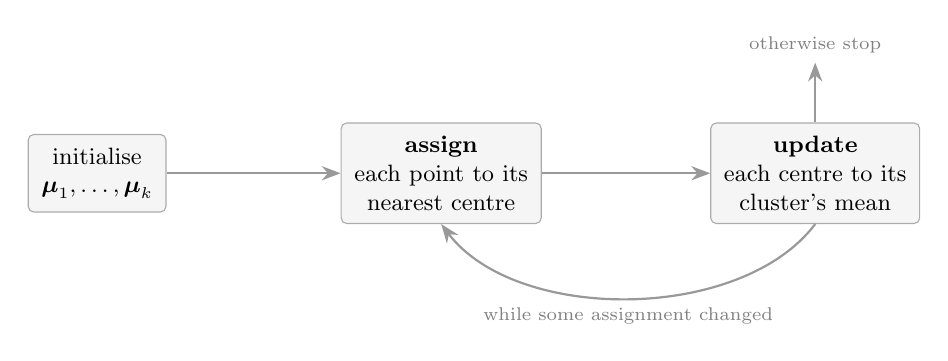
\begin{tikzpicture}[scale=0.95, every node/.style={transform shape}]
  \node[opbox,align=center] (init) at (0,0)
       {initialise\\$\bmu_1,\dots,\bmu_k$};
  \node[opbox,align=center] (asg)  at (4.6,0)
       {\textbf{assign}\\each point to its\\nearest centre};
  \node[opbox,align=center] (upd)  at (9.6,0)
       {\textbf{update}\\each centre to its\\cluster's mean};
  \draw[opar] (init) -- (asg);
  \draw[opar] (asg)  -- (upd);
  \draw[opar] (upd.south) .. controls (8.6,-2.0) and (5.6,-2.0) .. (asg.south)
        node[midway,below,font=\scriptsize,gray]
        {while some assignment changed};
  \draw[opar] (upd.north) -- ++(0,0.8)
        node[above,font=\scriptsize,gray]{otherwise stop};
\end{tikzpicture}
\end{center}

%------------------------------------------------------------------------------
\subsection{Pseudocode}
%------------------------------------------------------------------------------
\begin{algo}{$k$-means (Lloyd's algorithm)}
{\emph{Input:} data $\X=\{\vc{x}_1,\dots,\vc{x}_N\}\subseteq\R^{n}$; an integer
 $k$ with $1\le k\le N$. \quad\emph{Output:} centres
 $\bmu_1,\dots,\bmu_k$ and an assignment $a:\{1,\dots,N\}\to\{1,\dots,k\}$.}
  \item choose initial centres $\bmu_1,\dots,\bmu_k$
        \hfill\textit{\small e.g.\ $k$ distinct points of $\X$ at random}
  \item \kw{repeat}
  \item \ind \kw{for} $i=1$ \kw{to} $N$ \kw{do}
        \hfill\textit{\small assignment step}
  \item \indd $\displaystyle
        a(i) \;\leftarrow\; \argmin_{1\le j\le k}\ \norm{\vc{x}_i-\bmu_j}^{2}$
  \item \ind \kw{end for}
  \item \ind \kw{for} $j=1$ \kw{to} $k$ \kw{do}
        \hfill\textit{\small update step}
  \item \indd $\Cl_j \;\leftarrow\;
        \bigl\{\,\vc{x}_i \;:\; a(i)=j\,\bigr\}$
  \item \indd $\displaystyle
        \bmu_j \;\leftarrow\;
        \frac{1}{\lvert\Cl_j\rvert}\sum_{\vc{x}\,\in\,\Cl_j}\vc{x}$
        \hfill\textit{\small the mean, by \S11.5}
  \item \ind \kw{end for}
  \item \kw{until} no $a(i)$ changed during this pass
  \item \kw{return} $\bmu_1,\dots,\bmu_k$ and $a$
\end{algo}

\noindent That is the whole algorithm: two loops, one formula each. Line~4 is
$k$ distance comparisons; line~8 is an average. Nothing else happens.

\begin{rmk}
Line~4 uses $\norm{\cdot}^{2}$ rather than $\norm{\cdot}$, which is the shortcut
of \S7.5 arriving for the second time: the $\argmin$ depends only on the
ordering of the distances, squaring preserves that ordering, and so $Nk$ square
roots per iteration are avoided. Here there is an additional reason to prefer
the square, and it is not about speed --- $J$ itself is defined with squares, so
line~4 is minimising exactly the quantity the algorithm reports.
\end{rmk}

%------------------------------------------------------------------------------
\subsection{Why it stops}
%------------------------------------------------------------------------------
Nothing in the pseudocode obviously terminates: line~2 says ``repeat''. Here is
why it must.

\begin{itemize}[leftmargin=1.4em,itemsep=4pt]
  \item \textbf{Neither step can increase $J$.} The assignment step moves each
        point to a centre at least as close as its current one, so its
        contribution to $J$ does not rise. The update step replaces each centre
        by its cluster's mean, which by \S11.5 is the best possible centre for
        that cluster, so each cluster's contribution does not rise either.
  \item \textbf{There are finitely many assignments.} At most $k^{N}$ of them
        --- an enormous number, but a finite one. And each assignment determines
        its centres, hence determines $J$.
\end{itemize}

\noindent Put those together. If a pass changes some $a(i)$, then $J$ strictly
decreases, so that assignment can never recur. A sequence of strictly decreasing
values drawn from a finite set must stop, so after finitely many passes no
assignment changes and line~10 fires.

\begin{warn}[Terminating is not the same as being right]
The argument shows the algorithm halts and that it halts somewhere no single
step can improve. It does \emph{not} show it halts at the best clustering, and
in general it does not. What it reaches is a \emph{local} minimum: a
configuration where moving one point or nudging one centre makes things worse,
while some entirely different partition might have a far smaller $J$. \S14.1 is
about living with that.
\end{warn}

%------------------------------------------------------------------------------
\subsection{A worked example}
%------------------------------------------------------------------------------
\begin{ex}
Six points in $\R^{2}$, and $k=2$:
\[
  \vc{x}_1=[\,1,1\,],\quad \vc{x}_2=[\,2,1\,],\quad \vc{x}_3=[\,1,2\,],
  \qquad
  \vc{x}_4=[\,8,8\,],\quad \vc{x}_5=[\,9,8\,],\quad \vc{x}_6=[\,8,9\,].
\]
The two groups are obvious to the eye. To make the run interesting, initialise
\emph{badly}: put both centres inside the left-hand group,
\[
  \bmu_1 = [\,1,1\,], \qquad \bmu_2 = [\,2,1\,] .
\]

\subsubsection*{Iteration 1, assignment}
Squared distances to each centre, and the winner:

\begin{center}
\renewcommand{\arraystretch}{1.2}
\begin{tabular}{@{}l r r c@{}}
\toprule
\textbf{Point} & $\norm{\vc{x}-\bmu_1}^{2}$ & $\norm{\vc{x}-\bmu_2}^{2}$
  & $\boldsymbol{a(i)}$ \\
\midrule
$\vc{x}_1=[1,1]$ & $0$   & $1$   & $1$ \\
$\vc{x}_2=[2,1]$ & $1$   & $0$   & $2$ \\
$\vc{x}_3=[1,2]$ & $1$   & $2$   & $1$ \\
$\vc{x}_4=[8,8]$ & $98$  & $85$  & $2$ \\
$\vc{x}_5=[9,8]$ & $113$ & $98$  & $2$ \\
$\vc{x}_6=[8,9]$ & $113$ & $100$ & $2$ \\
\bottomrule
\end{tabular}
\end{center}

\noindent So $\Cl_1=\{\vc{x}_1,\vc{x}_3\}$ and
$\Cl_2=\{\vc{x}_2,\vc{x}_4,\vc{x}_5,\vc{x}_6\}$ --- a bad clustering, which is
what a bad initialisation buys.

\subsubsection*{Iteration 1, update}
\[
  \bmu_1 = \tfrac12\bigl([1,1]+[1,2]\bigr) = [\,1,\ 1.5\,],
  \qquad
  \bmu_2 = \tfrac14\bigl([2,1]+[8,8]+[9,8]+[8,9]\bigr)
             = \bigl[\,\tfrac{27}{4},\ \tfrac{26}{4}\,\bigr]
             = [\,6.75,\ 6.5\,] .
\]
The second centre has been dragged out of the left group towards the right one,
because four of its six points live there. At this stage
\[
  J = \underbrace{0.25+0.25}_{\Cl_1} + \underbrace{52.8125+3.8125+7.3125+7.8125}_{\Cl_2}
    = 72.25 .
\]

\subsubsection*{Iteration 2, assignment}
Recompute against the new centres $[\,1,1.5\,]$ and $[\,6.75,6.5\,]$:

\begin{center}
\renewcommand{\arraystretch}{1.2}
\begin{tabular}{@{}l r r c l@{}}
\toprule
\textbf{Point} & $\norm{\vc{x}-\bmu_1}^{2}$ & $\norm{\vc{x}-\bmu_2}^{2}$
  & $\boldsymbol{a(i)}$ & \\
\midrule
$\vc{x}_1=[1,1]$ & $0.25$   & $63.31$ & $1$ & \\
$\vc{x}_2=[2,1]$ & $1.25$   & $52.81$ & $1$ & \small(changed) \\
$\vc{x}_3=[1,2]$ & $0.25$   & $53.31$ & $1$ & \\
$\vc{x}_4=[8,8]$ & $91.25$  & $3.81$  & $2$ & \\
$\vc{x}_5=[9,8]$ & $106.25$ & $7.31$  & $2$ & \\
$\vc{x}_6=[8,9]$ & $105.25$ & $7.81$  & $2$ & \\
\bottomrule
\end{tabular}
\end{center}

\noindent One assignment changed --- $\vc{x}_2$ has come home --- so the loop
continues. Now
$\Cl_1=\{\vc{x}_1,\vc{x}_2,\vc{x}_3\}$ and
$\Cl_2=\{\vc{x}_4,\vc{x}_5,\vc{x}_6\}$.

\subsubsection*{Iteration 2, update}
\[
  \bmu_1 = \tfrac13\bigl([1,1]+[2,1]+[1,2]\bigr)
             = \bigl[\,\tfrac43,\ \tfrac43\,\bigr],
  \qquad
  \bmu_2 = \tfrac13\bigl([8,8]+[9,8]+[8,9]\bigr)
             = \bigl[\,\tfrac{25}{3},\ \tfrac{25}{3}\,\bigr] .
\]

\subsubsection*{Iteration 3, assignment}
Every point of the left group is now within squared distance $5/9$ of
$\bmu_1$ and more than $100$ from $\bmu_2$, and symmetrically on the
right. No assignment changes, so line~10 fires and the algorithm returns. The
final objective is
\[
  J = \underbrace{\tfrac29+\tfrac59+\tfrac59}_{\Cl_1}
    + \underbrace{\tfrac29+\tfrac59+\tfrac59}_{\Cl_2}
    = \tfrac{12}{9}+\tfrac{12}{9} = \tfrac83 \approx 2.67 .
\]
Against $72.25$ after the first pass, and monotonically decreasing throughout,
exactly as \S12.4 requires. \hfill$\blacksquare$
\end{ex}

\begin{center}
\begin{tikzpicture}[scale=0.55]
  \begin{scope}
    \draw[axisline] (-0.8,0) -- (11.5,0) node[right,font=\scriptsize,black]{$x_1$};
    \draw[axisline] (0,-0.8) -- (0,11.5) node[above,font=\scriptsize,black]{$x_2$};
    \foreach \x/\y in {1/1, 1/2} { \node[c1pt] at (\x,\y) {}; }
    \foreach \x/\y in {2/1, 8/8, 9/8, 8/9} { \node[c2pt] at (\x,\y) {}; }
    \node[cen1] at (1,1) {}; \node[cen2] at (2,1) {};
    \node[font=\scriptsize] at (5.6,-2.6) {after iteration 1's assignment};
  \end{scope}
  \begin{scope}[xshift=14cm]
    \draw[axisline] (-0.8,0) -- (11.5,0) node[right,font=\scriptsize,black]{$x_1$};
    \draw[axisline] (0,-0.8) -- (0,11.5) node[above,font=\scriptsize,black]{$x_2$};
    \foreach \x/\y in {1/1, 2/1, 1/2} { \node[c1pt] at (\x,\y) {}; }
    \foreach \x/\y in {8/8, 9/8, 8/9} { \node[c2pt] at (\x,\y) {}; }
    \node[cen1] at (1.3333,1.3333) {};
    \node[cen2] at (8.3333,8.3333) {};
    \node[font=\scriptsize] at (5.6,-2.6) {at termination};
  \end{scope}
\end{tikzpicture}
\end{center}

\noindent Stars are centres, discs are data points, and colour is the cluster
assignment. On the left both centres sit in the bottom corner and four points
have been swept into the red cluster; on the right each centre has settled at
the mean of its own group.

%==============================================================================
\section{What it costs}
%==============================================================================
Counting in FLOPs (\S4.6), for one iteration on $N$ points in $\R^{n}$ with $k$
clusters.

%------------------------------------------------------------------------------
\subsection{The assignment step}
%------------------------------------------------------------------------------
Line~4 computes, for each of the $N$ points, its squared distance to each of the
$k$ centres. One squared distance is $3n-1$ FLOPs by \S7.5 --- $n$ subtractions,
$n$ mults, $n-1$ adds --- so
\[
  \text{assignment} \;=\; Nk(3n-1) \text{ FLOPs} \;=\; O(Nkn) .
\]
Choosing the smallest of $k$ numbers is $k-1$ comparisons per point, $N(k-1)$ in
total, which is $O(Nk)$ and negligible beside $O(Nkn)$.

%------------------------------------------------------------------------------
\subsection{The update step}
%------------------------------------------------------------------------------
Line~8 totals each cluster and divides. Every point is added into exactly one
running total, and adding a vector of $\R^{n}$ costs $n$ adds (\S1.1), so all
the summing together is $Nn$ adds --- not $Nkn$, because each point belongs to
one cluster only. Then each of the $k$ centres is divided through by its size,
$n$ divisions each. So
\[
  \text{update} \;=\; Nn + kn \text{ FLOPs} \;=\; O(Nn) ,
\]
using $k\le N$. The update is cheaper than the assignment by a factor of $k$.

%------------------------------------------------------------------------------
\subsection{The total}
%------------------------------------------------------------------------------
Per iteration the assignment step dominates:
\[
  Nk(3n-1) + Nn + kn \;=\; O(Nkn) ,
\]
and if the algorithm runs for $T$ iterations,
\[
  \boxed{\;\text{$k$-means costs } O(T\,N\,k\,n) . \;}
\]

\begin{center}
\renewcommand{\arraystretch}{1.35}
\begin{tabular}{@{}l l l@{}}
\toprule
\textbf{Quantity} & \textbf{Cost} & \textbf{Comment} \\
\midrule
Assignment, one iteration & $O(Nkn)$   & $Nk$ distances of $O(n)$ each \\
Update, one iteration     & $O(Nn)$    & one pass over the data \\
One iteration             & $O(Nkn)$   & assignment dominates \\
Whole run                 & $O(TNkn)$  & $T$ = number of iterations \\
Memory                    & $O(Nn+kn)$ & the data, plus $k$ centres \\
\bottomrule
\end{tabular}
\end{center}

\noindent Linear in each of $N$, $k$, $n$ and $T$ separately, which is why the
algorithm scales to large datasets. Compare $k$-NN, which was $O(Nn)$ per
\emph{query} and had no training cost at all: $k$-means pays its cost once, up
front, and afterwards labelling a new point costs only $O(kn)$ --- the distance
to each of $k$ centres. It is an eager learner in the sense of \S7.4, where
$k$-NN is a lazy one.

\begin{rmk}[The one term that is not honest]
$T$ is doing something the other three are not. $N$, $k$ and $n$ are inputs you
know before you start; $T$ is however many iterations the algorithm happens to
need, which nobody knows in advance. In practice $T$ is small --- typically tens
--- and implementations cap it anyway with a maximum-iteration parameter. In
theory it can be far worse: examples are known where Lloyd's algorithm takes a
number of iterations exponential in $N$. Quoting $O(TNkn)$ and then treating $T$
as a modest constant is standard, and it is a convention rather than a theorem.
\end{rmk}

%==============================================================================
\section{What goes wrong}
%==============================================================================
%------------------------------------------------------------------------------
\subsection{Initialisation, and local minima}
%------------------------------------------------------------------------------
The example of \S12.5 recovered from a poor start. It need not have. Because
$J$ only ever decreases, the algorithm can never climb out of a bad basin it
falls into, and the clustering it returns can depend entirely on where the
centres began.

Two standard responses, and they are used together.

\begin{itemize}[leftmargin=1.4em,itemsep=4pt]
  \item \textbf{Restart.} Run the whole algorithm several times from different
        random initialisations and keep the run with the smallest final $J$.
        This multiplies the cost by the number of restarts and is worth it.
  \item \textbf{Initialise better.} Rather than choosing $k$ starting points
        uniformly at random, choose them to be spread out. That is
        \textbf{$k$-means++}, \S15.2, and it is the default everywhere.
\end{itemize}

%------------------------------------------------------------------------------
\subsection{Choosing $k$}
%------------------------------------------------------------------------------
The algorithm takes $k$ as an input, and the data rarely announces it.

\begin{warn}[You cannot choose $k$ by minimising $J$]
It is the obvious idea and it fails completely. $J$ decreases every time $k$
increases --- more centres means every point can be closer to one --- and at
$k=N$ every point is its own cluster and $J=0$. Minimising $J$ over $k$ always
returns $k=N$, which is not a clustering of anything.
\end{warn}

\noindent What is done instead:

\begin{itemize}[leftmargin=1.4em,itemsep=4pt]
  \item \textbf{The elbow method.} Plot $J$ against $k$. The curve falls
        steeply while $k$ is too small and then flattens once the real groups
        have been found; the ``elbow'' where the slope changes is taken as the
        answer. It is a judgement call read off a graph, and it is often
        ambiguous.
  \item \textbf{The silhouette score.} For each point, compare its average
        distance to its own cluster with its average distance to the nearest
        other cluster, and average the result over all points. Unlike $J$ this
        does not improve automatically with $k$, so it can be maximised.
  \item \textbf{Knowing the answer.} Often $k$ is set by the application --- a
        palette of $256$ colours, a marketing team that can run four campaigns
        --- and no statistics are needed.
\end{itemize}

%------------------------------------------------------------------------------
\subsection{The shape assumption}
%------------------------------------------------------------------------------
Look again at line~4: a point joins the cluster whose centre is nearest. That
single line decides the geometry of everything the algorithm can produce. The
set of points closer to $\bmu_j$ than to any other centre is bounded by flat
surfaces --- the perpendicular bisectors between centres --- so \emph{$k$-means
always cuts the space into straight-sided convex pieces}. It is structurally
incapable of returning a cluster shaped like a ring or a crescent, however
obvious that shape is to the eye.

It also has a size preference. A large, spread-out cluster contributes more to
$J$ than a small tight one, so the algorithm tends to split genuine large
clusters and merge genuine small ones in order to balance the total.

\begin{rmk}
When the clusters are not blob-shaped, the fix is to change algorithm rather
than to tune this one. The $k$-NN graph methods of \S9.3 --- spectral
clustering, DBSCAN --- group points that are connected by chains of short hops
and have no convexity assumption at all, which is exactly the case $k$-means
cannot handle. The two families are complementary, and knowing which failure
you are looking at is most of the skill.
\end{rmk}

%------------------------------------------------------------------------------
\subsection{Two smaller traps}
%------------------------------------------------------------------------------
\begin{itemize}[leftmargin=1.4em,itemsep=4pt]
  \item \textbf{Empty clusters.} If no point is nearest to $\bmu_j$, then
        $\Cl_j=\varnothing$ and line~8 divides by zero. Implementations detect
        this and reseed the orphaned centre, usually onto the point currently
        furthest from its own centre.
  \item \textbf{Feature scaling.} Everything said in \S8.2 applies here without
        modification and for the same reason: $J$ is a sum of squared Euclidean
        distances, so a feature measured in large units dominates it and
        silently decides the clustering. Standardize first.
\end{itemize}

%==============================================================================
\section{In practice}
%==============================================================================
%------------------------------------------------------------------------------
\subsection{Where it is used}
%------------------------------------------------------------------------------
\begin{center}
\renewcommand{\arraystretch}{1.4}
\begin{tabular}{@{}l >{\raggedright\arraybackslash}p{9.4cm}@{}}
\toprule
\textbf{Application} & \textbf{The vectors, and what a cluster means} \\
\midrule
Colour quantization
  & Each pixel of an image is a point in $\R^{3}$, its red, green and blue
    values. Cluster them with $k=256$ and repaint every pixel in its centroid's
    colour: the image now uses $256$ colours instead of millions. This is how a
    GIF palette is built. \\
Vector quantization
  & The same idea in compression generally. The centroids form a
    \emph{codebook}, and each data vector is transmitted as the index of its
    nearest centroid rather than as itself. \\
Customer segmentation
  & Each customer is a vector of behaviours; the clusters are groups to be
    treated alike. Probably the most common commercial use. \\
Document grouping
  & Documents embedded as vectors; clusters are topics, discovered rather than
    specified. \\
Anomaly detection
  & Cluster the normal data, then score a new point by its distance to the
    nearest centroid. Large distance, suspicious point --- at a cost of
    $O(kn)$, not $O(Nn)$. \\
Indexing for search
  & $k$-means partitions the space into cells; a nearest-neighbour query then
    searches only the few cells nearest the query rather than all $N$ points.
    This is the \texttt{IVF} index of \S10.2 --- $k$-means is the machinery
    inside the $k$-NN speed-up. \\
\bottomrule
\end{tabular}
\end{center}

\noindent The last row is worth pausing on. Part 2 listed IVF among the ways to
make nearest-neighbour search fast without saying how the cells were built. They
are built by running this algorithm. The two parts of this unit are not merely
adjacent topics; one is a component of the other.

%------------------------------------------------------------------------------
\subsection{Making it better and faster}
%------------------------------------------------------------------------------
\subsubsection*{$k$-means\texttt{++}: a better start}
Choose the first centre uniformly at random from $\X$. Then choose each
subsequent centre at random from $\X$ as well, but with point $\vc{x}$ weighted
by $D(\vc{x})^{2}$, where $D(\vc{x})$ is the distance from $\vc{x}$ to the
nearest centre already chosen. Points far from everything chosen so far are
therefore likely to be picked next, and the initial centres come out spread
across the data rather than clumped.

This costs $O(Nkn)$ --- one extra iteration's worth --- and it buys a genuine
guarantee: the expected final $J$ is within a factor of $O(\log k)$ of the true
optimum, which is more than plain Lloyd's offers, namely nothing. It has been
the default initialisation since Arthur and Vassilvitskii introduced it in 2007.

\subsubsection*{Skipping distances with the triangle inequality}
The assignment step recomputes all $Nk$ distances every iteration, and most of
that work is wasted: after the first few passes, almost every point keeps the
cluster it had. The following lemma lets those be detected without measuring.

\begin{lem}[Elkan]
Let $d$ be a metric and let $\vc{x}$, $\vc{b}$, $\vc{c}$ be points. If
$d(\vc{b},\vc{c}) \ge 2\,d(\vc{x},\vc{b})$, then
$d(\vc{x},\vc{c}) \ge d(\vc{x},\vc{b})$.
\end{lem}

\begin{proof}
By the triangle inequality \textbf{M4} of the vector unit, \S14.1,
$d(\vc{b},\vc{c}) \le d(\vc{b},\vc{x}) + d(\vc{x},\vc{c})$. Rearranging and
using the hypothesis,
\[
  d(\vc{x},\vc{c}) \;\ge\; d(\vc{b},\vc{c}) - d(\vc{x},\vc{b})
                   \;\ge\; 2\,d(\vc{x},\vc{b}) - d(\vc{x},\vc{b})
                   \;=\; d(\vc{x},\vc{b}) . \qedhere
\]
\end{proof}

\noindent Read $\vc{b}$ as the centre $\vc{x}$ currently belongs to and
$\vc{c}$ as some other centre. The lemma says: if the two centres are at least
twice as far apart as $\vc{x}$ is from its own, then $\vc{c}$ cannot be closer,
and the distance $d(\vc{x},\vc{c})$ need never be computed. Since the $k$
centre-to-centre distances change slowly, they can be computed once per
iteration --- $O(k^{2}n)$ --- and used to skip a large fraction of the $Nk$
point-to-centre distances. Elkan's algorithm (2003) and Hamerly's (2010) do
exactly this, with caches of upper and lower bounds, and are often several times
faster while returning \emph{identical} results.

\begin{rmk}
That lemma is the second time in this unit that a metric axiom has paid for
itself computationally --- the first was the same pruning applied to $k$-NN in
\S10.2. It is worth noticing what kind of fact \textbf{M4} turns out to be. In
the vector unit it looked like a sanity condition, the formal version of ``the
direct route is not longer''. Here it is the thing that lets a program decline
to do arithmetic, and it works for \emph{any} metric, which is why the same
trick appears in two different algorithms.
\end{rmk}

\subsubsection*{Mini-batch $k$-means}
Instead of using all $N$ points each iteration, draw a random sample of size $b
\ll N$ and update the centres from that. Each iteration costs $O(bkn)$ rather
than $O(Nkn)$. The result is slightly worse and it arrives orders of magnitude
sooner, which is the right trade for datasets that do not fit in memory.

\subsubsection*{$k$-medoids}
Replace the centroid of line~8 with the medoid of \S11.4. The centres are then
guaranteed to be actual data points, and the method inherits the medoid's
resistance to outliers --- at a considerably higher cost, since a medoid needs
pairwise distances. The classical algorithm is \textbf{PAM} (Partitioning Around
Medoids). Use it when averaging your vectors would produce nonsense.

%------------------------------------------------------------------------------
\subsection{What the industry uses}
%------------------------------------------------------------------------------
\begin{center}
\renewcommand{\arraystretch}{1.35}
\begin{tabular}{@{}l >{\raggedright\arraybackslash}p{9.0cm}@{}}
\toprule
\textbf{Tool} & \textbf{What it is} \\
\midrule
\texttt{scikit-learn}
  & \texttt{KMeans}, with $k$-means\texttt{++} initialisation and Elkan's
    algorithm both available as defaults, plus \texttt{MiniBatchKMeans}. The
    teaching and prototyping standard. \\
\texttt{FAISS}
  & Meta's \texttt{faiss.Kmeans}, built for millions of vectors and GPU
    execution. Used to build the IVF cells of \S10.2. \\
Spark \texttt{MLlib}
  & Distributed $k$-means for data spread across a cluster of machines, where
    the update step becomes a map-reduce over partitions. \\
\texttt{cuML}
  & NVIDIA's GPU implementation, for when the whole dataset fits in
    video memory. \\
\bottomrule
\end{tabular}
\end{center}

\noindent Every one of these is line-for-line the pseudocode of \S12.3, with a
better first line and an assignment step that avoids arithmetic it can prove is
unnecessary. The algorithm itself has not changed since Lloyd described it in
1957.

\lookahead Both algorithms in this unit reduce to the same two operations:
measure distances between vectors, and average vectors. Both were counted with
the tools of Part 1 and both live in the floating-point set of \S3. What neither
can do is change the space the data lives in --- and \S8.3 already noted that in
high dimension the distances they rely on stop discriminating. Fixing that means
finding a better basis for the data, which requires the objects of the matrix
unit and, eventually, the singular value decomposition. That is the direction
the rest of the course takes.

\end{document}
